\documentclass[a4paper]{scrreprt}
\usepackage[top=2.2cm, bottom=3.5cm]{geometry}
\usepackage{listings}
\usepackage{underscore}
\usepackage{graphicx}
\usepackage{xcolor}
\usepackage{longtable}
\usepackage{tabularx}   
\usepackage{fancyhdr}
\usepackage{subcaption}
\usepackage[bookmarks=true]{hyperref}
\usepackage[utf8]{inputenc}
\usepackage[english]{babel}
\graphicspath{{../app_screenshots/}}
\hypersetup{
    bookmarks=false,    % show bookmarks bar?
    pdftitle={Software Requirement Specification},    % title
    pdfauthor={Wong Chu Feng},                     % author
    pdfsubject={TeX and LaTeX},                        % subject of the document
    pdfkeywords={TeX, LaTeX, graphics, images}, % list of keywords
    colorlinks=true,       % false: boxed links; true: colored links
    linkcolor=blue,       % color of internal links
    citecolor=black,       % color of links to bibliography
    filecolor=black,        % color of file links
    urlcolor=purple,        % color of external links
    linktoc=page            % only page is linked
}%
\def\myversion{0.9.0}
\date{}
% \title{}
\usepackage{hyperref}

\begin{document}
% Set the footer style for the current page only
\fancypagestyle{currentpagefooter}{
    \fancyfoot[C]{Copyright © 1999 by Karl E. Wiegers. Permission is granted to use, modify, and distribute this document.}
    \renewcommand{\headrulewidth}{0pt}
    \renewcommand{\footrulewidth}{0pt}
}
\thispagestyle{currentpagefooter}

\begin{flushright}
    \rule{16cm}{5pt}\vskip2cm
    \begin{bfseries}
        \Huge{SOFTWARE REQUIREMENTS\\ SPECIFICATION}\\
        \vspace{3.5cm}
        for\\
        \vspace{1.5cm}
        Glucometer App\\
        \vspace{3.2cm}
        \LARGE{Version \myversion}\\
        \vspace{1.5cm}
        Prepared by : Wong Chu Feng\\
        \vspace{1.5cm}
        Trilogy Technologies Pte Ltd\\
        \vspace{1.5cm}
        21 July 2023\\
    \end{bfseries}
\end{flushright}
\clearpage

\chapter*{Revision History}
\begin{center}
\begin{longtable}{|p{2.8cm}|l|p{7cm}|l|}
    \hline
    \textbf{Name} & \textbf{Date} & \textbf{Description} & \textbf{Version} \\
    \hline
    Glucometer connectivity integration & 10 May 2023 & The app currently includes a splash screen and establishes BLE connection to the glucometer, enabling data exchange and monitoring between the app and the glucometer. & 0.5 \\
    \hline
    Add Personal Information page and bug fix & 22 May 2023 & Added a page for users to key in their personal information which includes their name, age, gender, height, and weight. Fixed a bug that prevented the saving of entered personal information. & 0.5.1\\
    \hline
    Export and Storage options & 23 May 2023 & Users can now choose to export and save biodata as .xls or .csv into their mobile phone storage. Fixed an issue where the exported file could not be saved. & 0.6 \\
    \hline
    Add email function & 23 May 2023 & Users can choose to send the saved data via email  & 0.6.1\\
    \hline
    Basic graph display & 25 May 2023 & Added the most basic graph that reads data from the local database and plots a graph to display all the data. & 0.7\\
    \hline
    Graph package update & 26 March 2023 & Updated graph package from charts_flutter to syncfusion_flutter_charts due to deprecation. & 0.8\\
    \hline
    System compatibility & 1 June 2023 & Migrated app from Android 8.0 to Android 10.0, including necessary dependency updates. & 0.8.0.1\\
    \hline
    Graph display and data format fixes & 8 June 2023 & Fixed DateTime format to ensure proper graph display. Resolved a problem with time format when inserting data into the database. & 0.8.1\\
    \hline
    iOS Development & 12 June 2023 & Built iOS development app using Xcode 13. & 0.8.2\\
    \hline
    Dashboard enhancement & 15 June 2023 & Created a new, visually appealing dashboard to display biodata & 0.8.3\\
    \hline
    BLE compatibility improvement & 22 June 2023 & Fixed problem where newer devices cannot deteect BLE device. & 0.8.4\\
    \hline  
    Data filtering and graph visualisation & 28 June 2023 & Users are now able to filter the data and view their data on the graph by the day, week, month, or year. & 0.8.5\\
    \hline
    Refactor code & 29 June 2023 & This version change focuses on code refactoring, primarily to improve readability of the code base. This reorganization streamlines the development process, increase code efficiency and ensures a more robust foundation for future enhancements to any component in the app. & 0.8.5.1\\
    \hline
    Graph colour highlighting & 30 June 2023 & Graph now visually highlights glucose levels above the threshold. & 0.8.5.2\\
    \hline
    Multi-language support & 11 July 2023 & Added multi-language support for English, Mandarin, Malay, Hindi and Tamil. & 0.9.0\\
    \hline
\end{longtable}
\end{center}


\tableofcontents


\chapter{Introduction}

\section{Purpose}
The Glucometer App serves as a comprehensive digital companion, enabling users to record and track essential health metrics such as heart rate, cholesterol level, uric acid level, glucose level and SpO2 level.
\newline
With user-friendly features like data storage and data sharing with healthcare professionals and visual trend analysis through graphs, this app paves the way to revolutionise and elevate the current state of teleconsultation and remote health monitoring between patients and doctors.
\newline
By providing a convenient and efficient platform for tracking and sharing essential health metrics, it bridges the gap between individuals and healthcare providers, enabling more informed and personalised remote consultations.

\section{Document Conventions}\begin{itemize}
    \item Glucometer
    \begin{itemize}
        \item A blood glucose meter is a (medical) device used to measure the concentration of glucose in a person’s blood. It is commonly used by diabetic patients to monitor their glucose levels.
        \item Specific to Trilogy Technologies’ glucometer, it can measure not only glucose levels but also uric acid, heartrate, SpO2, and cholesterol levels.
        \item The Arduino code defines the healthy range to be $<140mg/dl$ or $<7.8mmol/l$.
    \end{itemize}
    
    \item SpO2
    \begin{itemize}
        \item The measurement of oxygen saturation in a person’s blood. It generally should range from 96\% - 99\%.
    \end{itemize}

    \item Cholesterol
    \begin{itemize}
        \item The fatty substance found in our bodies which can cause health issues in excess.
        \item The Arduino code defines the healthy range to be $<200mg/dl$ or $<6.6mmol/l$
    \end{itemize}

    \item Uric Acid (UA)
    \begin{itemize}
        \item A waste product produced by the body's metabolism of certain foods. Elevated UA levels can lead to health issues.
        \item The Arduino code defines a healthy range for both men and women.
        \item Range for men: $[4.0, 8.5]$ in $mg/dl$ or $[0.24, 0.51]$ in $mmol/l$
        \item Range for women: $[2.7, 7.3]$ in $mg/dl$ or $[0.16, 0.43]$ in $mmol/l$
    \end{itemize}

    \item MAX30100 PulseOximeter
    \begin{itemize}
        \item Heart rate sensor module that measures heart rate.
    \end{itemize}

    \item Adafruit SSD1306
    \begin{itemize}
        \item Organic light-emitting diode (OLED) graphic display.
    \end{itemize}

    \item Bluetooth Low Energy (BLE)
    \begin{itemize}
        \item A wireless communication technology designed for energy-efficient data exchange between devices. More commonly used in devices that transmits data over short distances.
        \item Unlike traditional Bluetooth, BLE is more optimised for low-power, less data-intensive applications where energy efficiency is crucial, making it ideal for devices that require intermittent data exchange or have limited power.
        \item No direct connection is required resulting in significant battery power savings. Instead, the app listens for the broadcast from the glucometer and hones onto the signal emitted from the BLE device to receive the data.
        \item Note: BLE connection does not work on an emulator.
    \end{itemize}
    \end{itemize}
This SRS document is adapted from the IEEE standard for Software Requirements Specification.


\section{Intended Audience and Reading Suggestions}
This SRS document serves as a blueprint for developers and testers.
\newline
Developers can understand the purpose of this project and find any necessary information about the requirements or functionality of the app through this document. A clear description of the development process will be described and made easy for any to follow along.
\newline
Extending from this understanding to testers, they are able to identify the test cases that need to be executed to ensure the app can carry out its desired function. Test scenarios and test cases are to help validate the functionality and performance of the app.


\section{Project Scope}
Glucometer App is a user-friendly free-of-charge application that targets diabetic patients or those at risk and encompasses a range of features designed to empower users in monitoring and managing their glucose levels and aiding their healthcare providers.
\newline
This app serves as a digital health companion, enabling users to effortlessly view their glucose levels. With a user-friendly interface, users can securely store their data or conveniently email it to their healthcare provider for analysis and consultation, all done within the app. The app also incorporates an interactive graph, allowing users to visually track and analyse their glucose level over time, fostering a better understanding of their health status and facilitating informed decision-making regarding lifestyle choices or treatment plans.
\newline
However, this app will not provide medical advice, nor will it replace the guidance of a healthcare professional.
\newline


\chapter{Overall Description}

\section{Product Perspective}
The Glucometer app fits into a broader healthcare ecosystem, playing a pivotal role in empowering individuals to manage their health effectively. Within this perspective, the app interacts with various entities, including Trilogy Technologies’ glucometers for data recording and input, user devices such as smartphones for data storage and communication channels for data sharing with healthcare professionals.
\newline
Furthermore, it aligns with prevailing privacy regulations and data protection measures to safeguard sensitive health information. By considering the app’s place within a larger ecosystem, it ensures a seamless user-centric approach to health management.

\section{Product Functions}
\begin{itemize}
    \item App must record and monitor heart rate, glucose level, cholesterol level, uric acid level and SpO2 levels.
    \item Users must be able to save their personal information including but not limited to name, age, gender, height and weight.
    \item App must provide the function to export and save biodata as .xls or .csv files to mobile phone storage.
    \item App must provide the function to email biodata saved as .xls and .csv files.
    \item App must allow users to filter and view their recorded data on a graph by day, week, month, or year.
    \item The graph must be visually appealing and provide color coding to highlight glucose levels above the set threshold.
    \item App must offer seamless connectivity with compatible glucometers for data input.
    \item App must be compatible on both Android and iOS platforms.
    \item User experience must be enhanced with visually appealing and intuitive dashboard to view their biodata while recording with the glucometer.
\end{itemize}

\section{User Classes and Characteristics}
\begin{itemize}
    \item Regular users
    \begin{itemize}
        \item Frequency of use: Regular and frequent use of the app
        \item Subset of product functions: Utilise all product functions for comprehensive health monitoring and data management.
        \item Technical expertise: Varying technical proficiency levels.
        \item Security level: Standard user privileges with access to only their own personal data.
        \item Education level/Experience: Diverse educational backgrounds.
    \end{itemize}
    \item Healthcare professionals
    \begin{itemize}
        \item Frequency of use: Periodic use for reviewing patient data and providing medical advice.
        \item Subset of product functions: Access and analyse user-submitted data for medical evaluation and consultation.
        \item Technical expertise: High level of proficiency in digital health tools and analysing health-related data.
        \item Security level: Enhanced access privileges to view and analyse multiple users' data.
        \item Education level/Experience: Qualified healthcare professionals with relevant medical training and expertise.
    \end{itemize}
    \item Technical support team
    \begin{itemize}
        \item Frequency of use: Occasional use for troubleshooting and providing technical assistance.
        \item Subset of product functions: Focus on addressing technical issues, software updates and user support.
        \item Technical expertise: Advanced technical knowledge to troubleshoot app-related problems.
        \item Security level: Access to system logs and user support resources.
        \item Education level/Experience: Technical professionals with expertise in app development and support.
    \end{itemize}
\end{itemize}


\section{Operating Environment}
The app will support both Android and iOS platforms. 

\section{User Documentation}
A demonstration video and app screenshots alongside this SRS documentation will be uploaded so prospective users are able to understand how to use the app.

\section{Assumptions and Dependencies}
\begin{itemize}
    \item Users must be connected to Wi-Fi or mobile data and have a device that supports Bluetooth connectivity.
    \item Users must use a mobile device that is either on Android or iOS platforms to download the app.
    \item The app will support English, Mandarin, Malay, Hindi and Tamil languages.
    \item The app is only designed for mobile phone usage.
\end{itemize}

\chapter{External Interface Requirements}
\section{User Interfaces}
The app features a personal information page that includes fields that accepts user input where the system only accepts a valid value. For example, the 'age' field must only accept values in $[0, 120]$, 'height' field must be between $(0, 272]$, etc.
\newline
\subsection{Personal Information page}
This page includes fields where the user is able to key in his/her own information. Each detail can be changed and saved accordingly.

\begin{itemize}
    \item Users can click on the input text box and type in the respective values and select their gender from 2 options, Male or Female.
    \item To save the data, they will click on the ‘Save’ button and the data will always appear there even after they have navigated to another tab. To change the input data, they just have to click on the box, retype in a new data and click on ‘Save’.
    \item The data will always appear there even after they have navigated to another tab.
\end{itemize}

\begin{figure}[h]
    \centering
    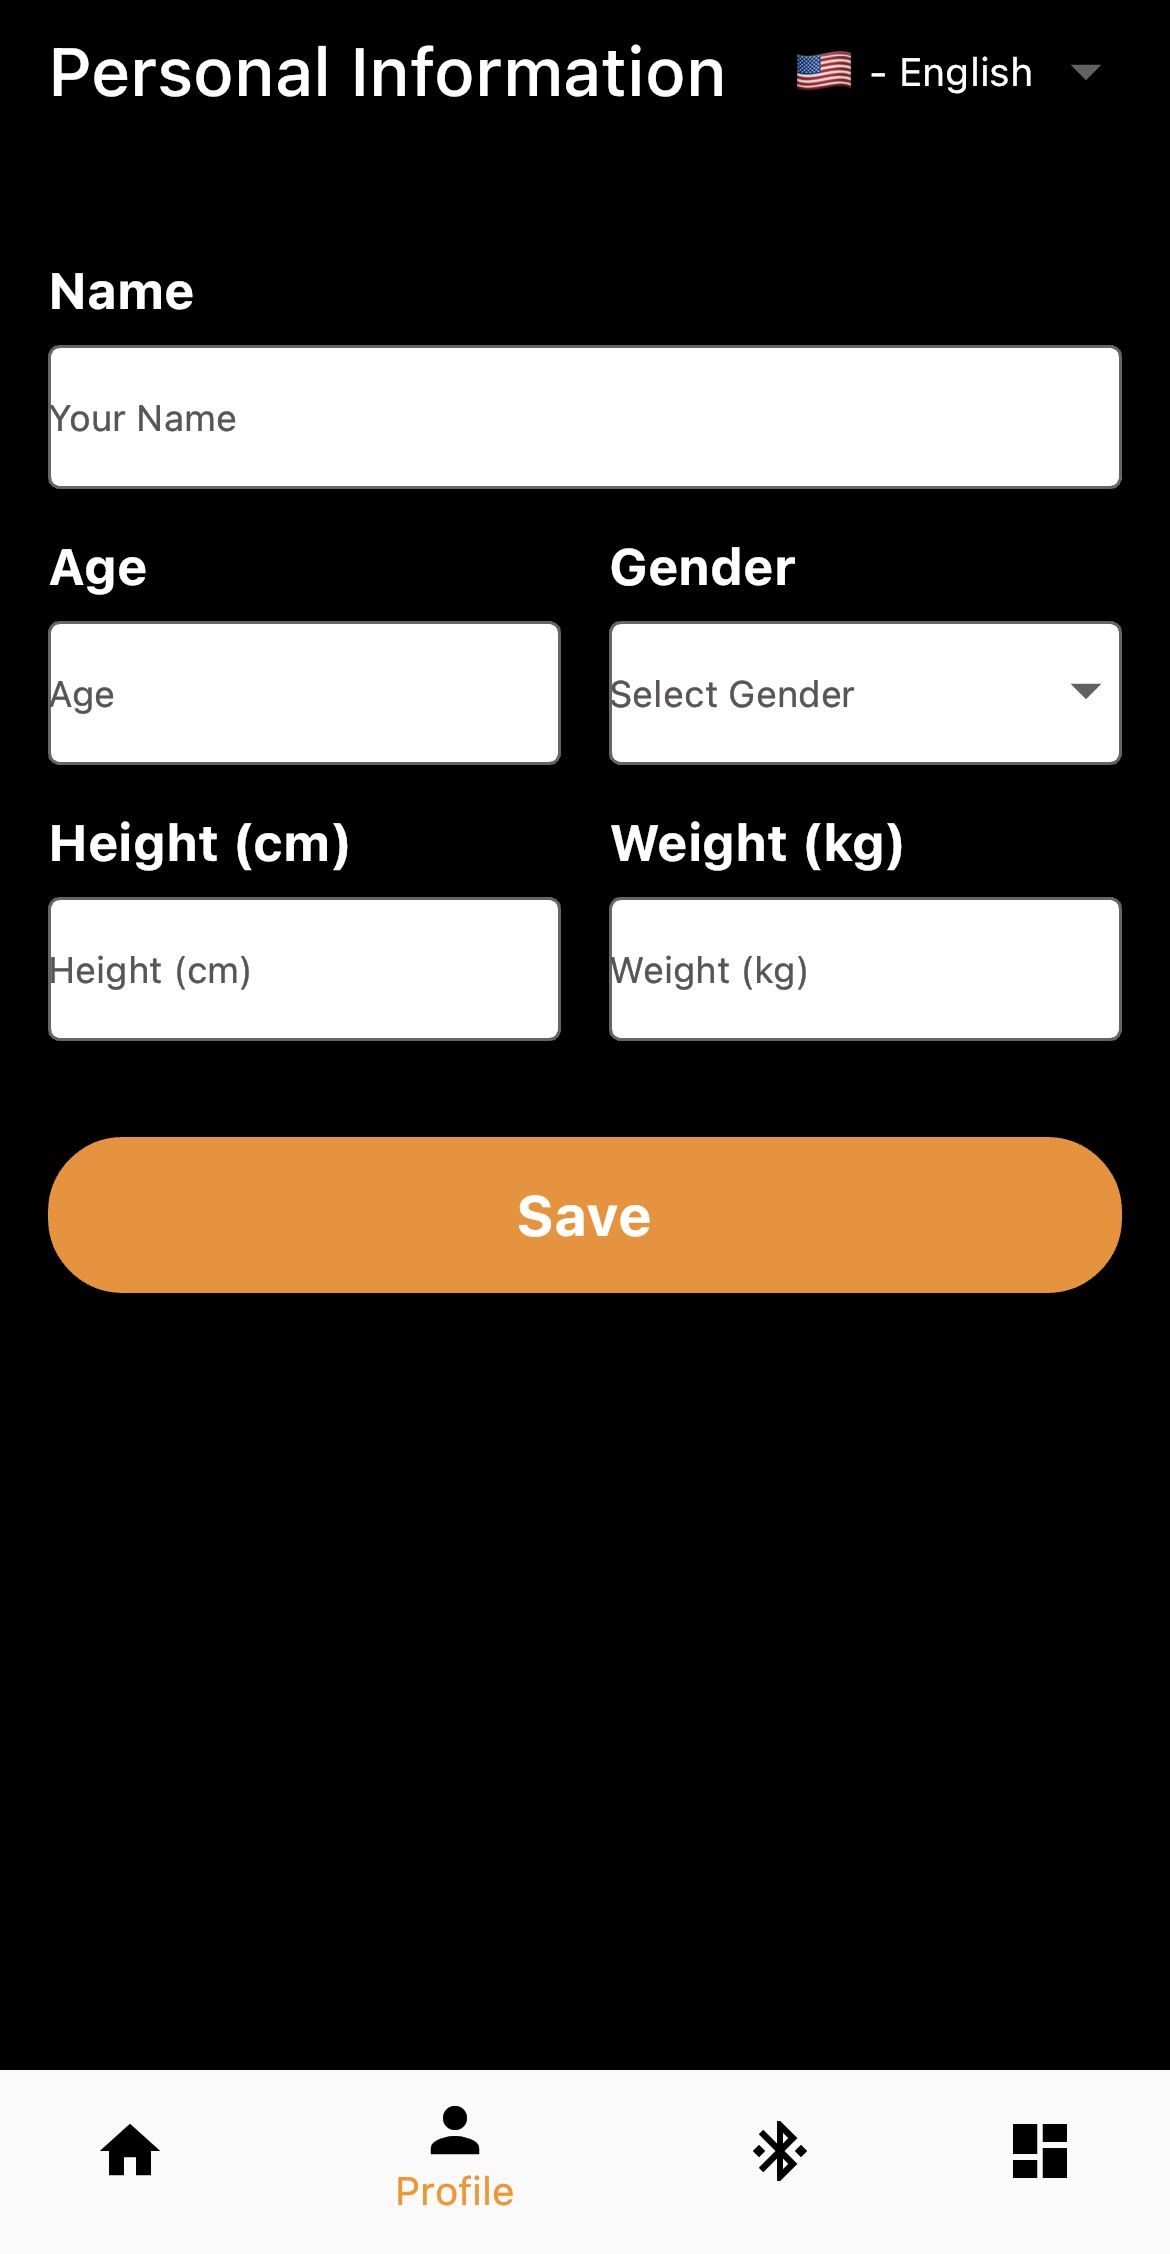
\includegraphics[scale=0.125]{personal_info.png}
    \caption{Personal Information page}
    \label{fig:personal-info}
\end{figure}
\clearpage

\vspace*{4.2cm}
\begin{figure}[htbp]
    \centering
    \begin{subfigure}{0.45\textwidth}
        \centering
        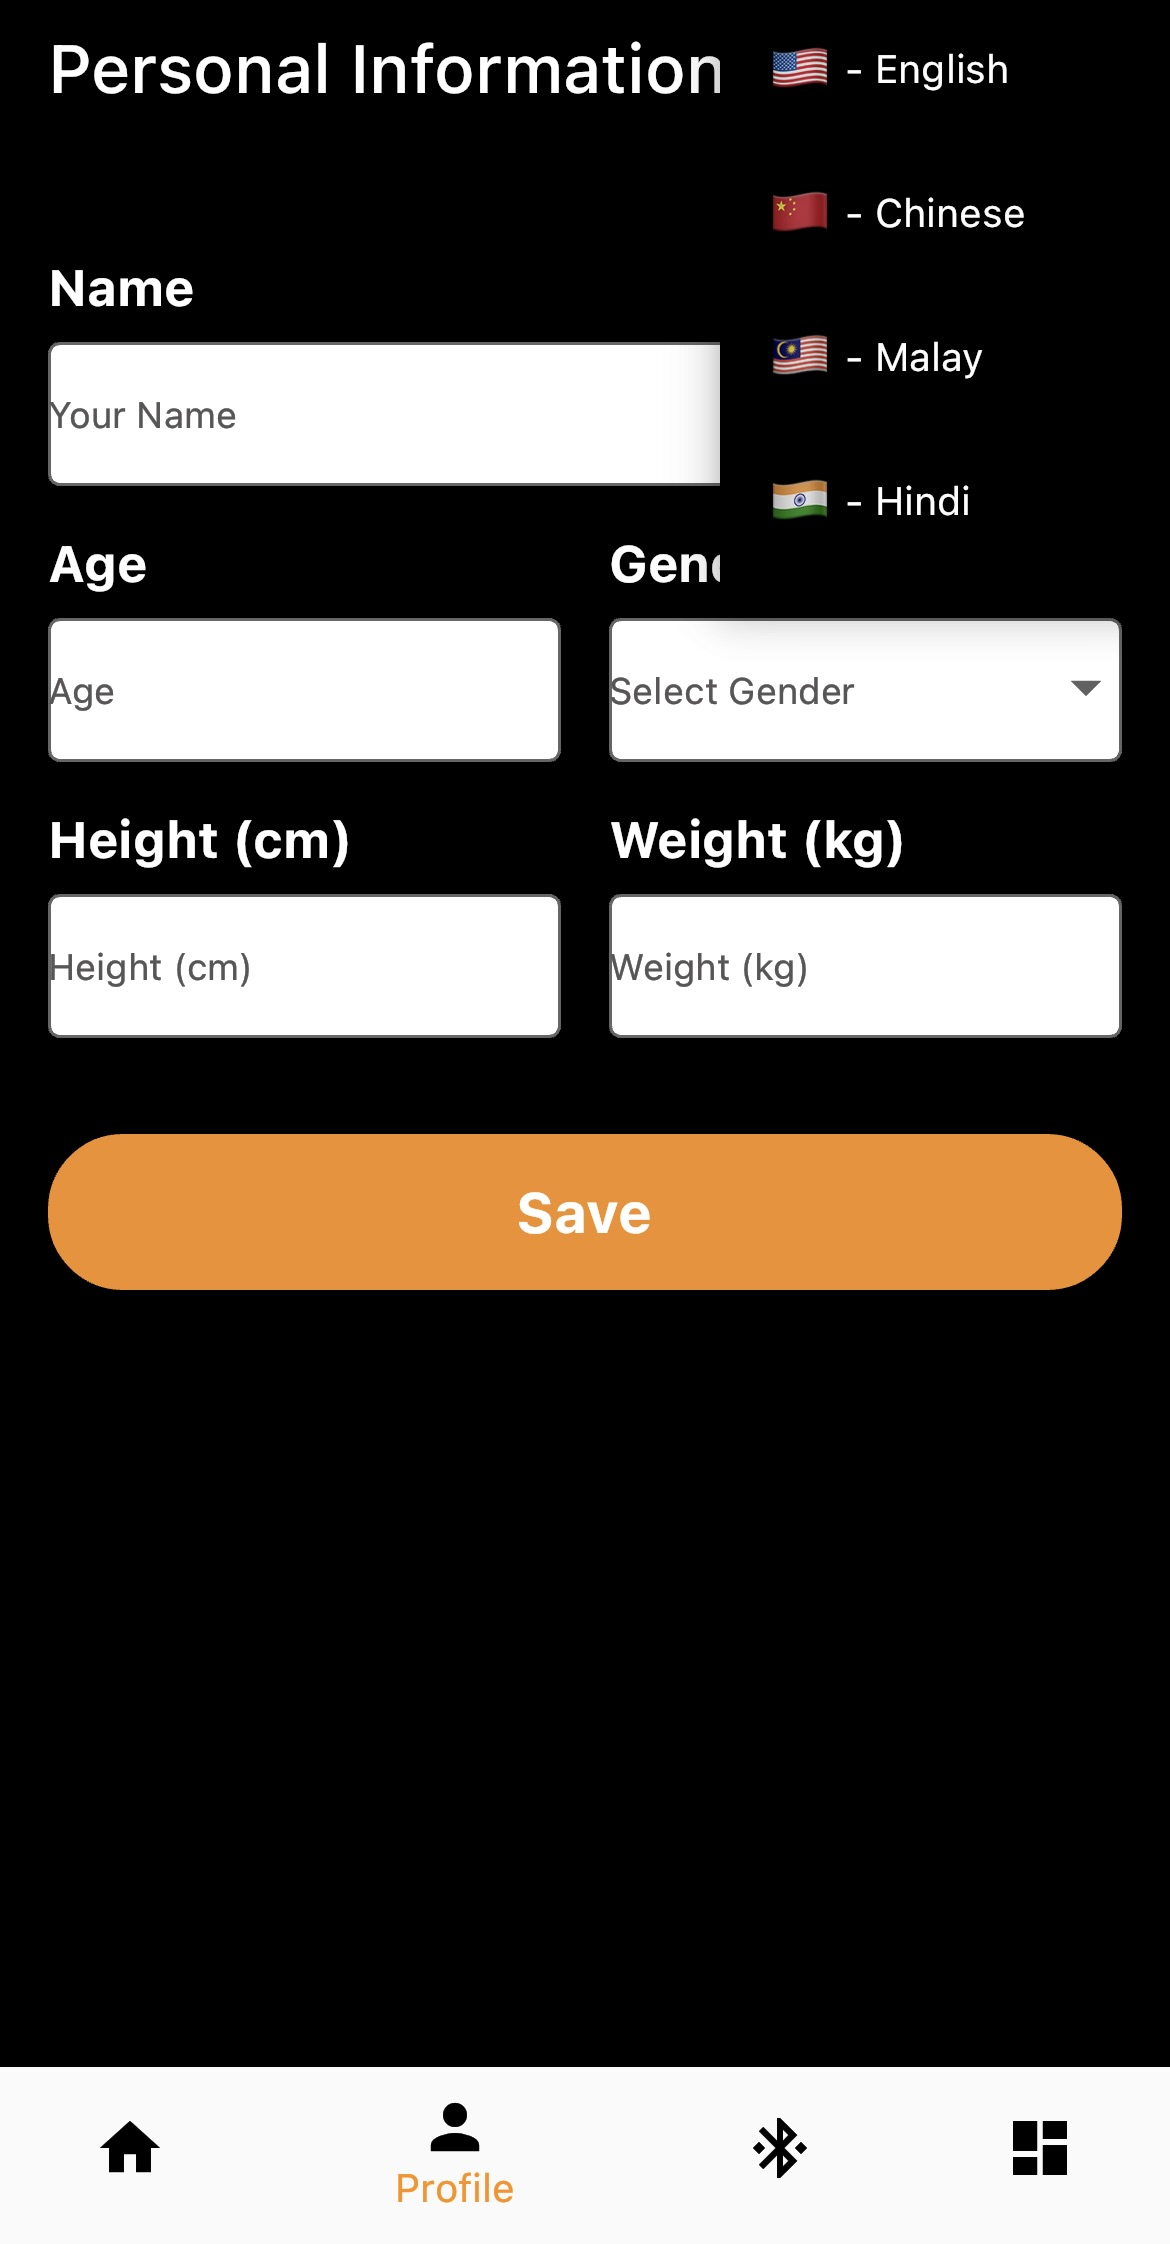
\includegraphics[scale=0.15]{languages_all.jpeg}
        \caption{All languages}
        \label{fig:graph1}
    \end{subfigure}
    \begin{subfigure}{0.45\textwidth}
        \centering
        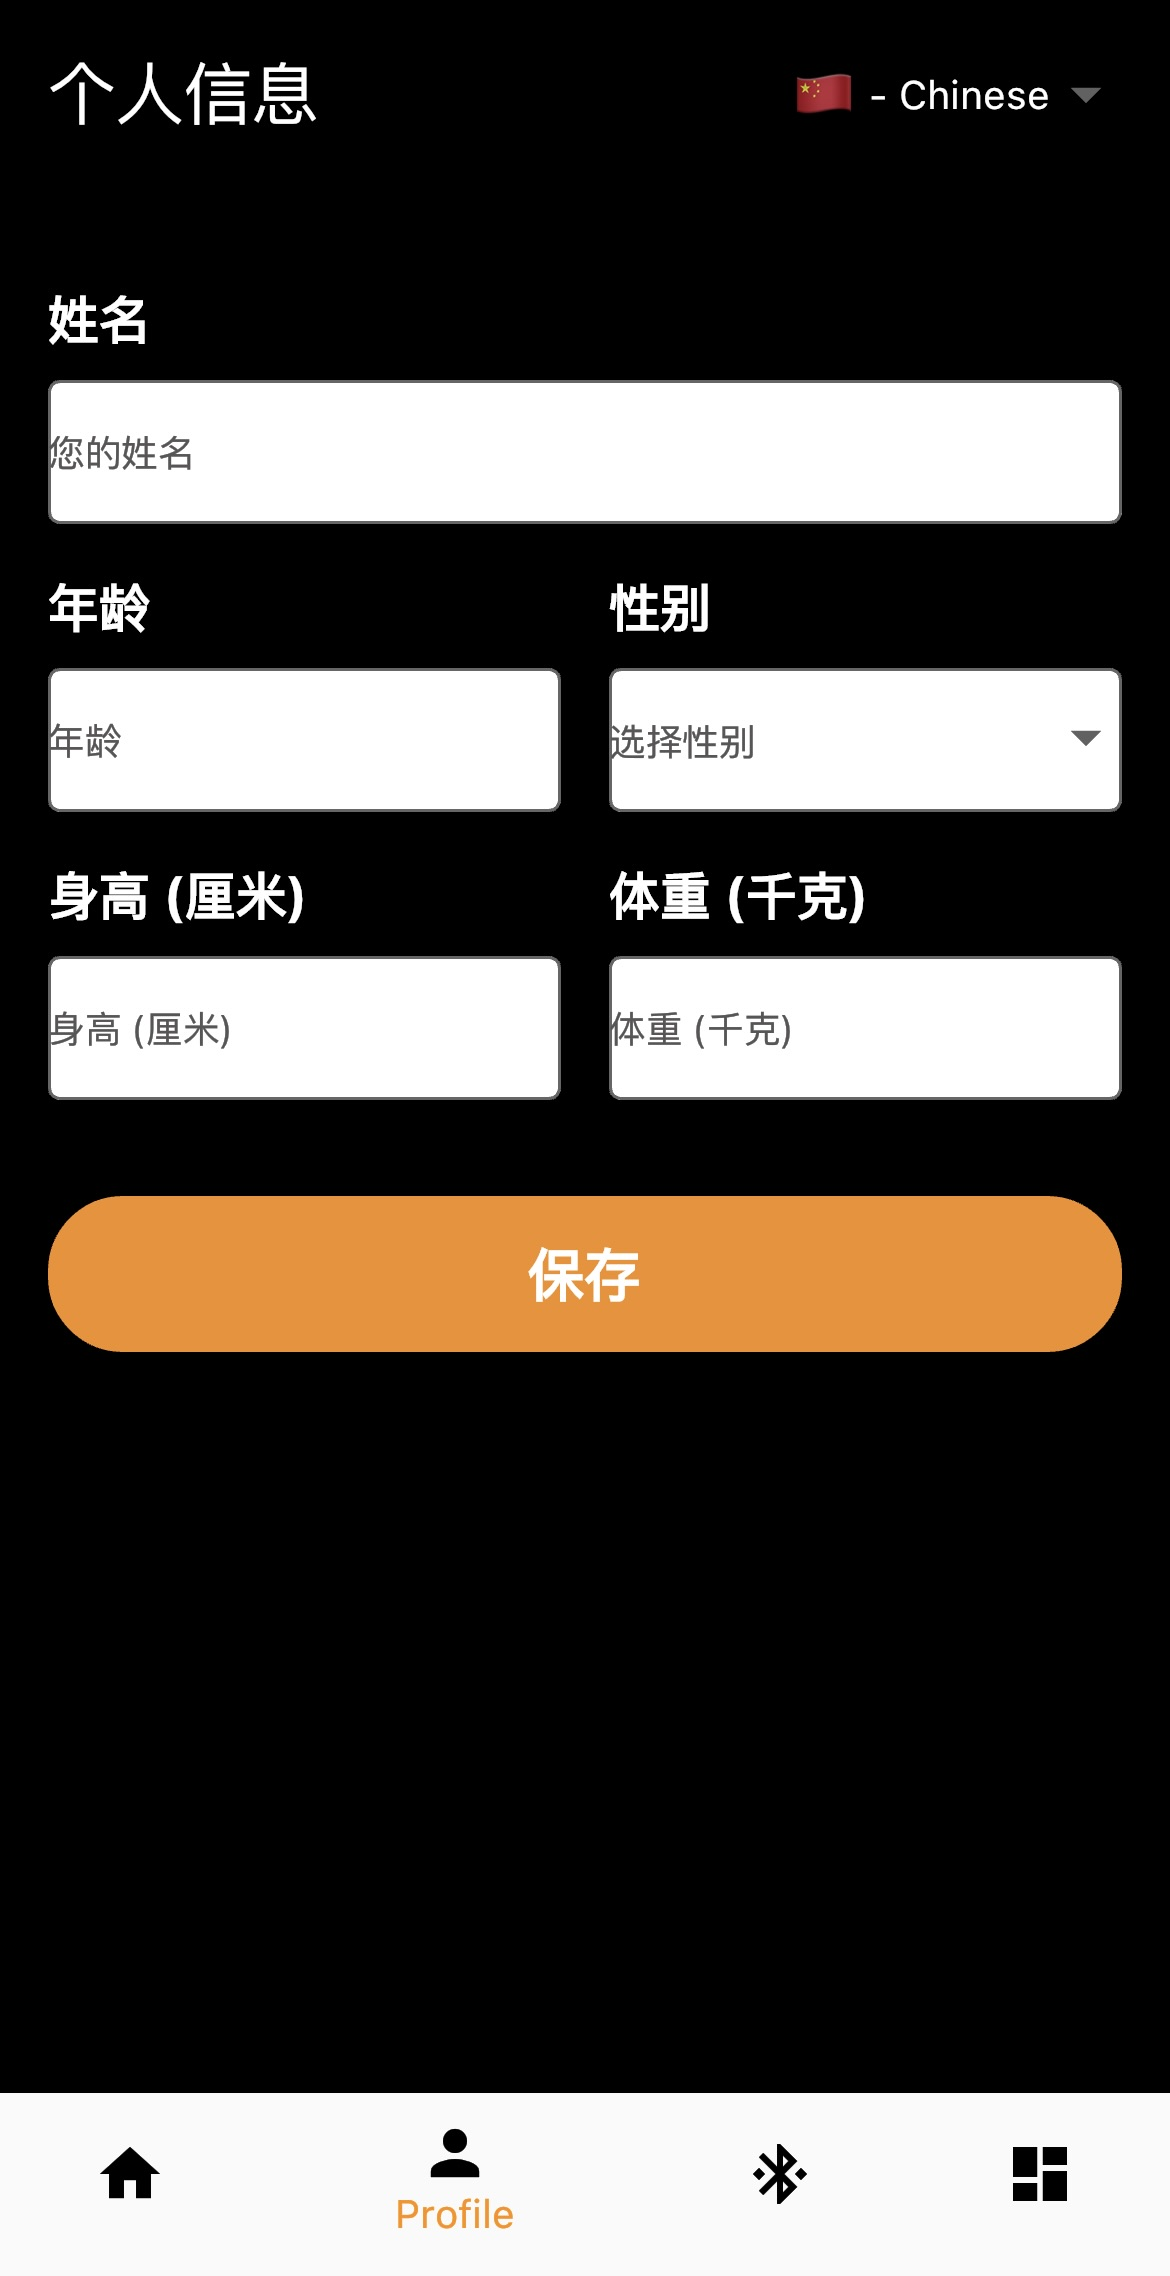
\includegraphics[scale=0.15]{languages_chinese.jpeg}
        \caption{Example: Chinese}
        \label{fig:graph2}
    \end{subfigure}
    \label{fig:finddev}
\end{figure}
\clearpage

\subsection{Find Devices page}
This page will be where the user search for the oximeter. The live updates of the biodata received will be redirected to the next Dashboard page.
\newline
When a device is connected in 3.1.2(a), a row of data containing the variables that are being measured is displayed. They include heart rate, blood oxygen level, glucose level, cholesterol level, men uric acid level and women uric acid level.
\newline
\begin{figure}[htbp]
    \centering
    \begin{subfigure}{0.45\textwidth}
        \centering
        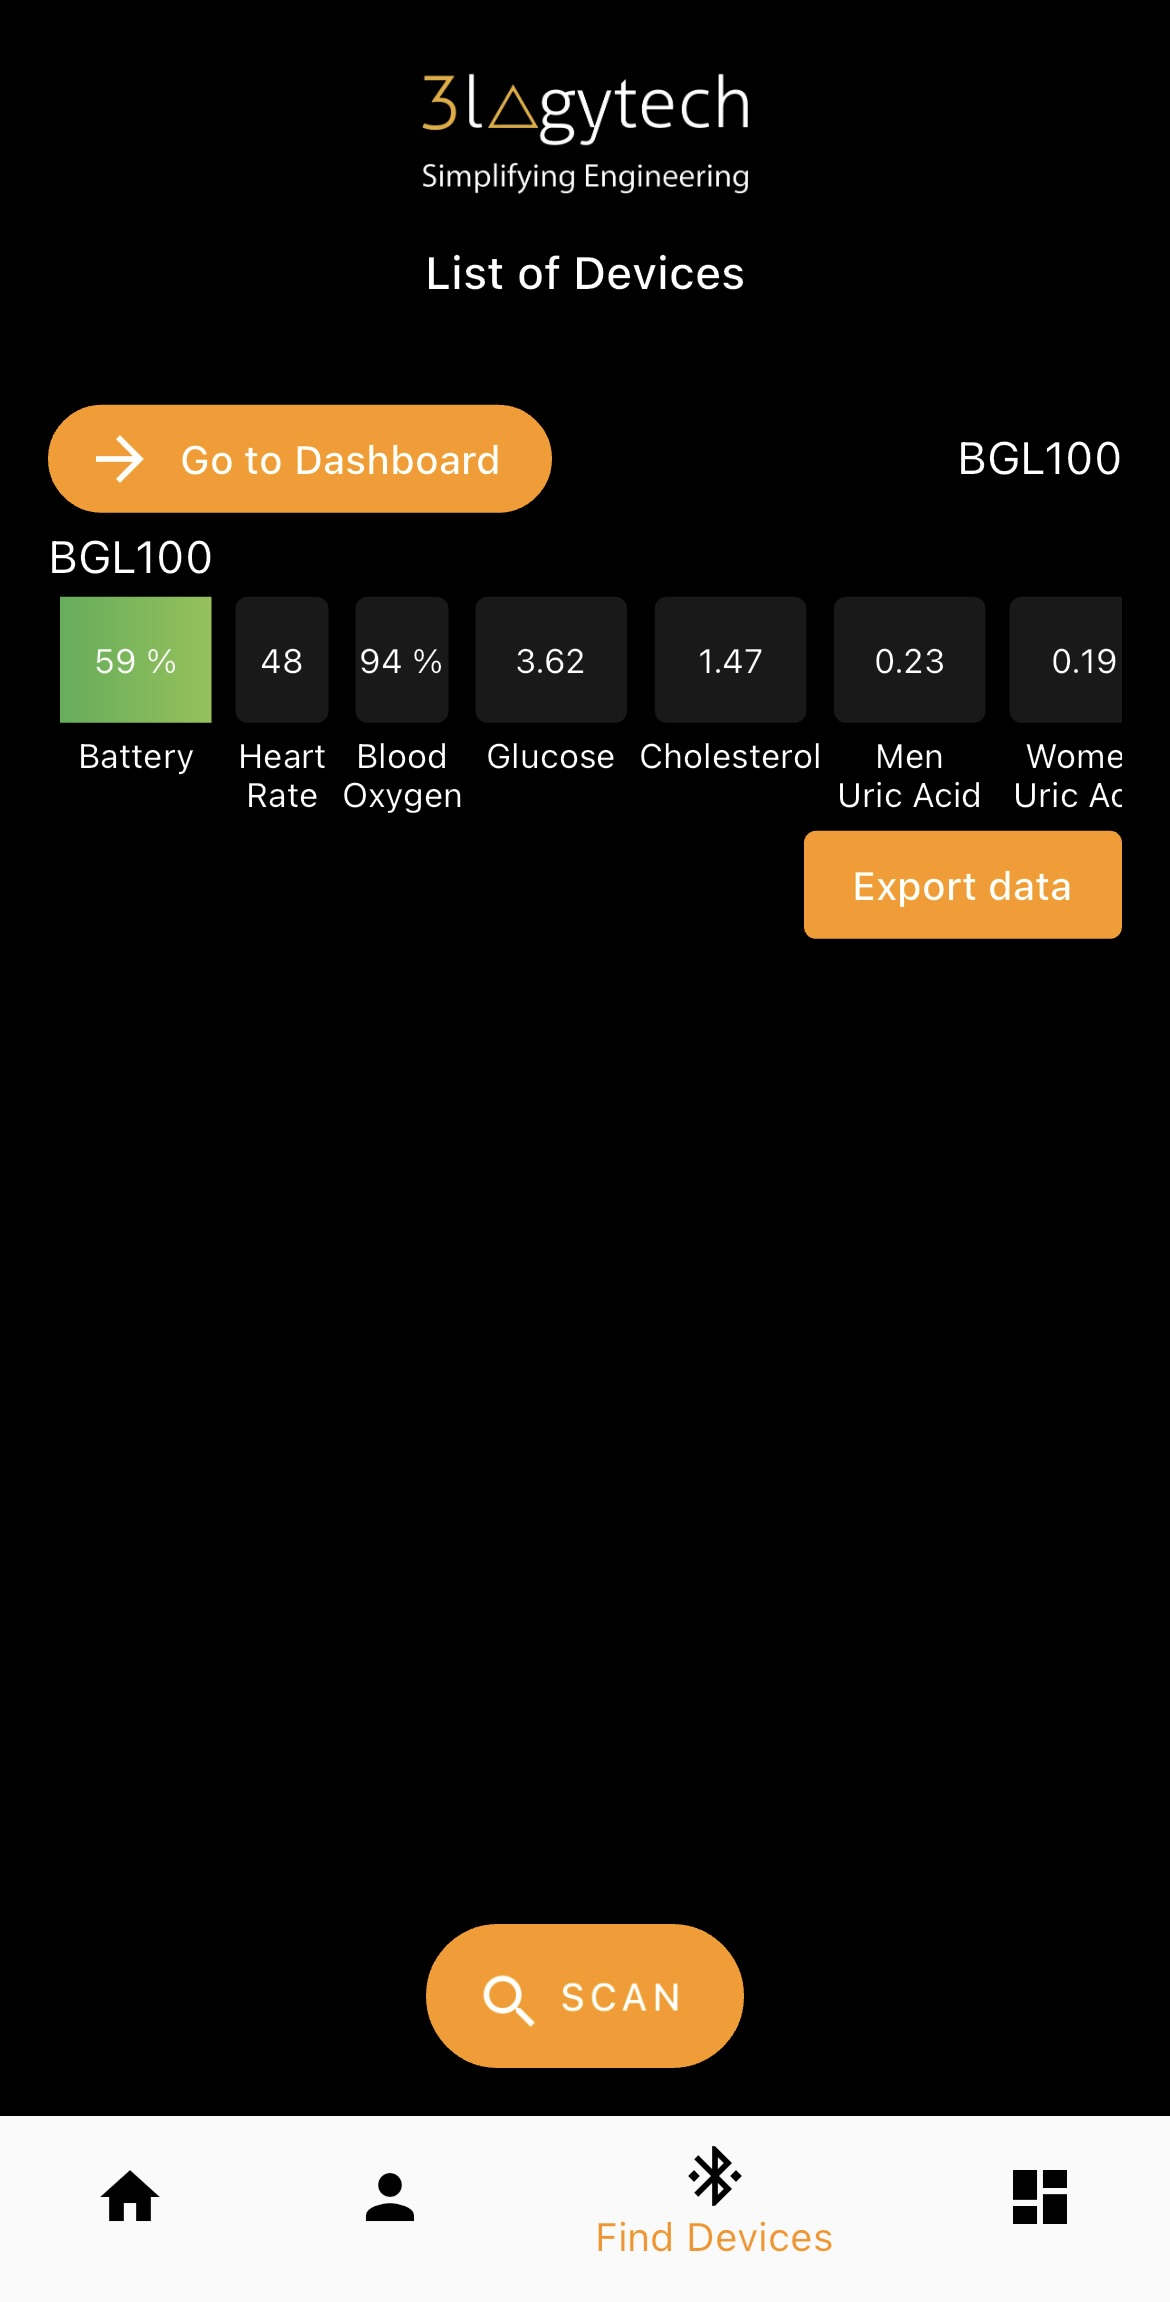
\includegraphics[scale=0.15]{find_devices.jpeg}
        \caption{Device connected}
        \label{fig:graph1}
    \end{subfigure}
    \begin{subfigure}{0.45\textwidth}
        \centering
        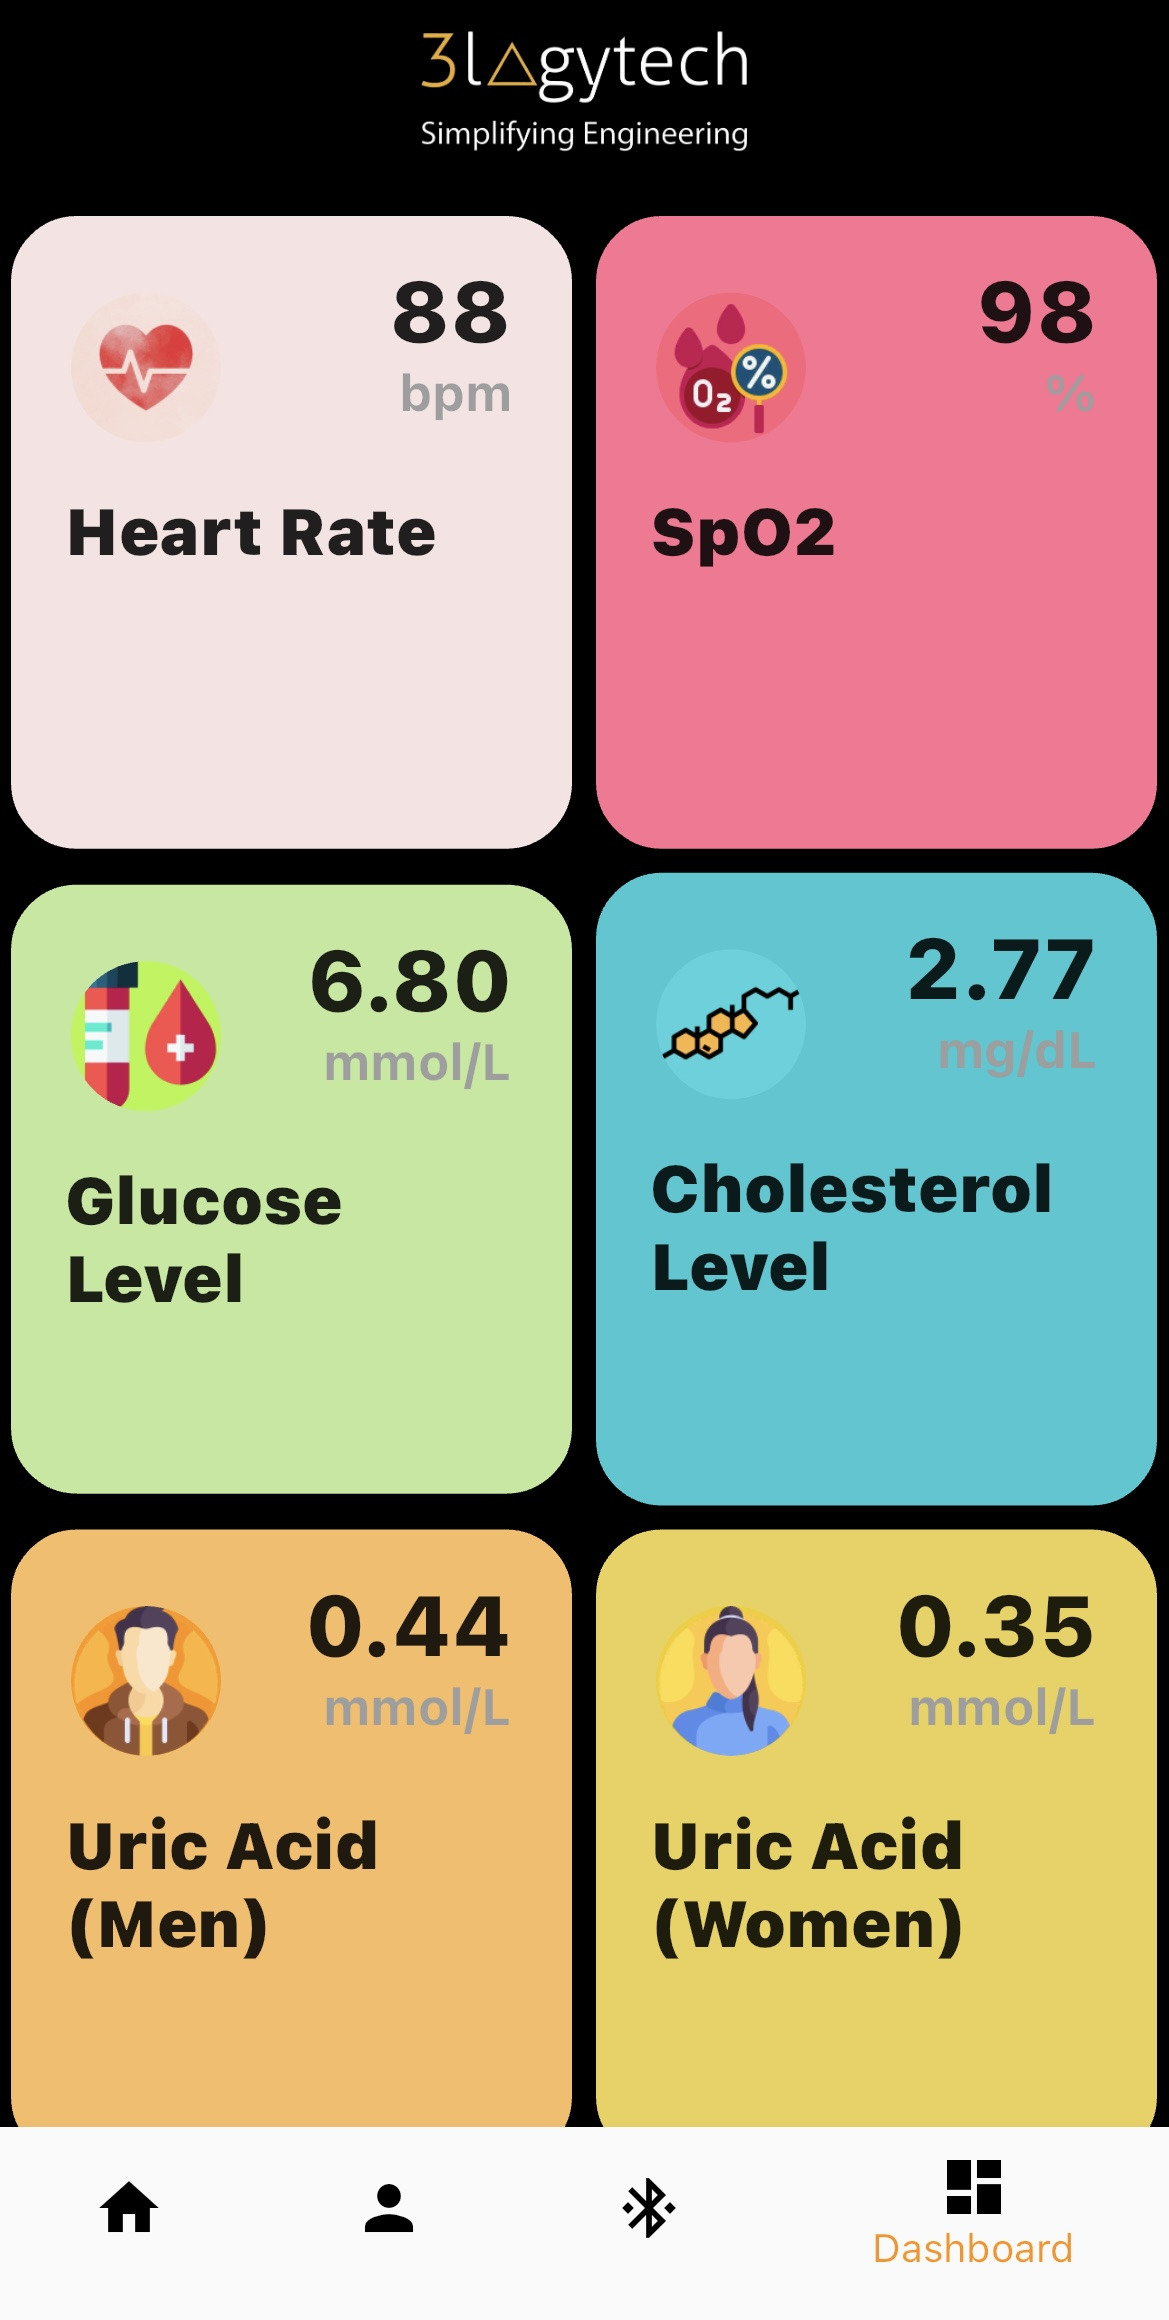
\includegraphics[scale=0.15]{dashboard_data.jpeg}
        \caption{Dashboard with data}
        \label{fig:graph2}
    \end{subfigure}
    \label{fig:finddev}
\end{figure}
\clearpage

\subsubsection{3.1.2.1 Export data}
To export data, the user will click on the 'Export data' button. The data will be exported into either .xls or .csv.
\newline
\newline
The first 2 options:
\begin{itemize}
    \item Exports the data and saves into the phone’s local storage as a CSV file or an Excel file.
\end{itemize}
The last 2 options:
\begin{itemize}
    \item Emails the data in either as a CSV file or an Excel file. The file will also be saved into the phone’s local storage automatically.
\end{itemize}
\begin{figure}[htbp]
    \centering
    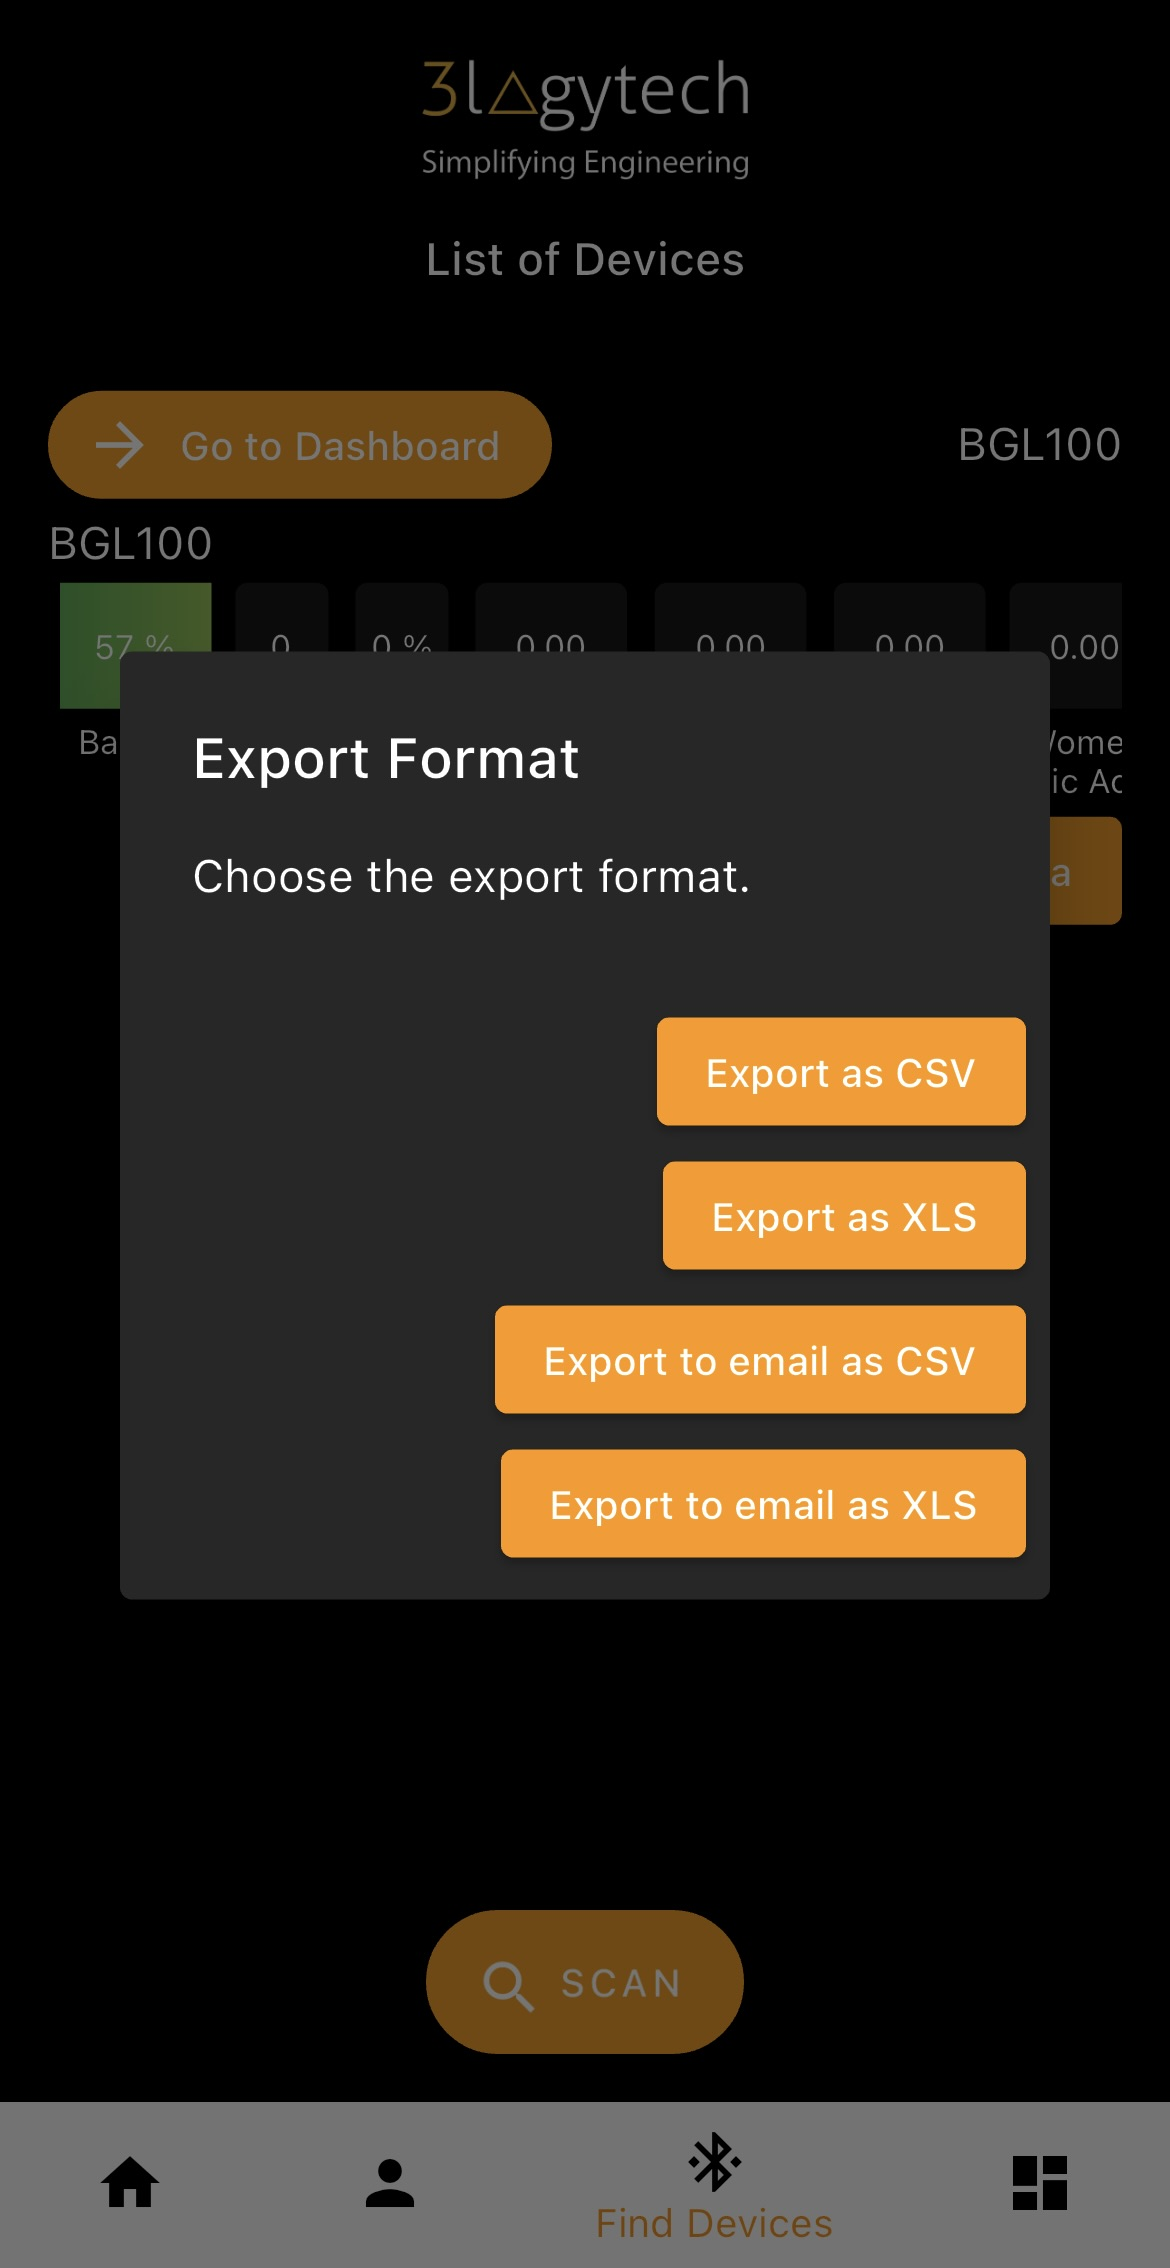
\includegraphics[scale=0.15]{export_page.jpeg}
    \caption{Export dialogue}
\end{figure}
\clearpage

\subsection{Graph page}
This page will be where the user search for the oximeter. The live updates of the biodata received will be redirected to the next Dashboard page.
\begin{figure}[h]
    \centering
    \begin{subfigure}{0.45\textwidth}
        \centering
        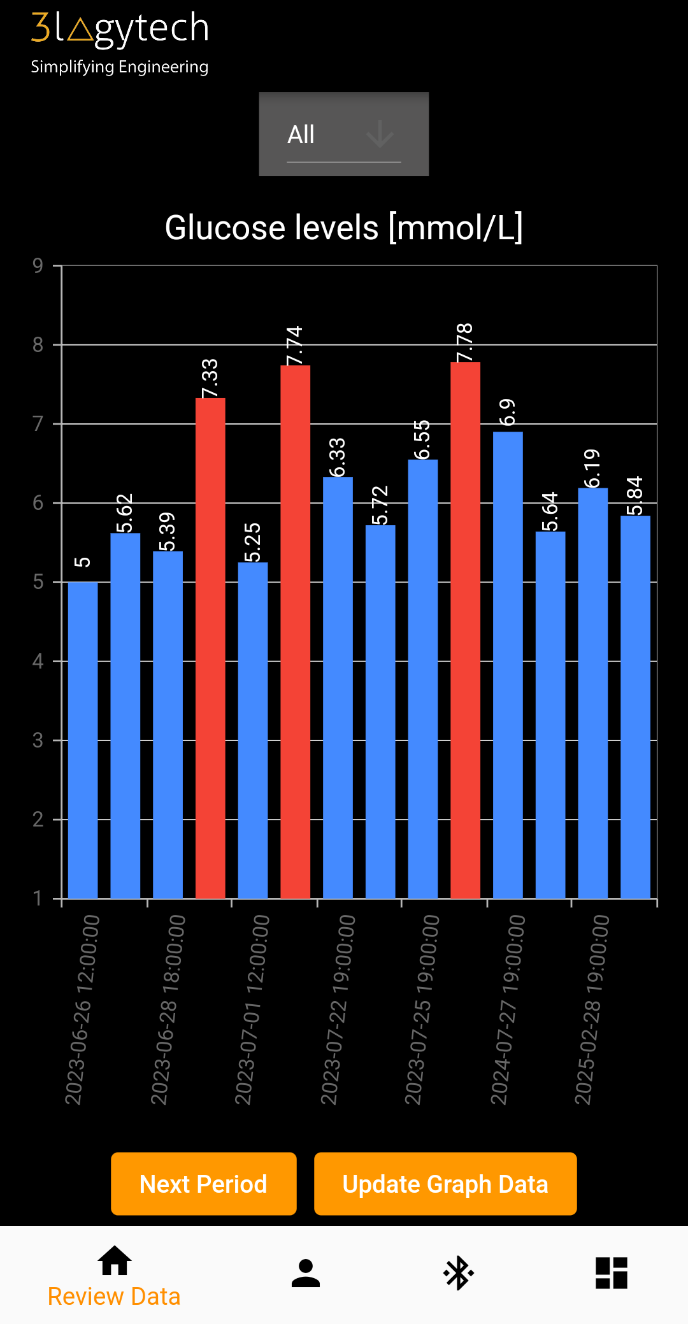
\includegraphics[scale=0.5]{graph_all.png}
        \caption{Graph showing 'All' data}
        \label{fig:graph1}
    \end{subfigure}
    \begin{subfigure}{0.45\textwidth}
        \centering
        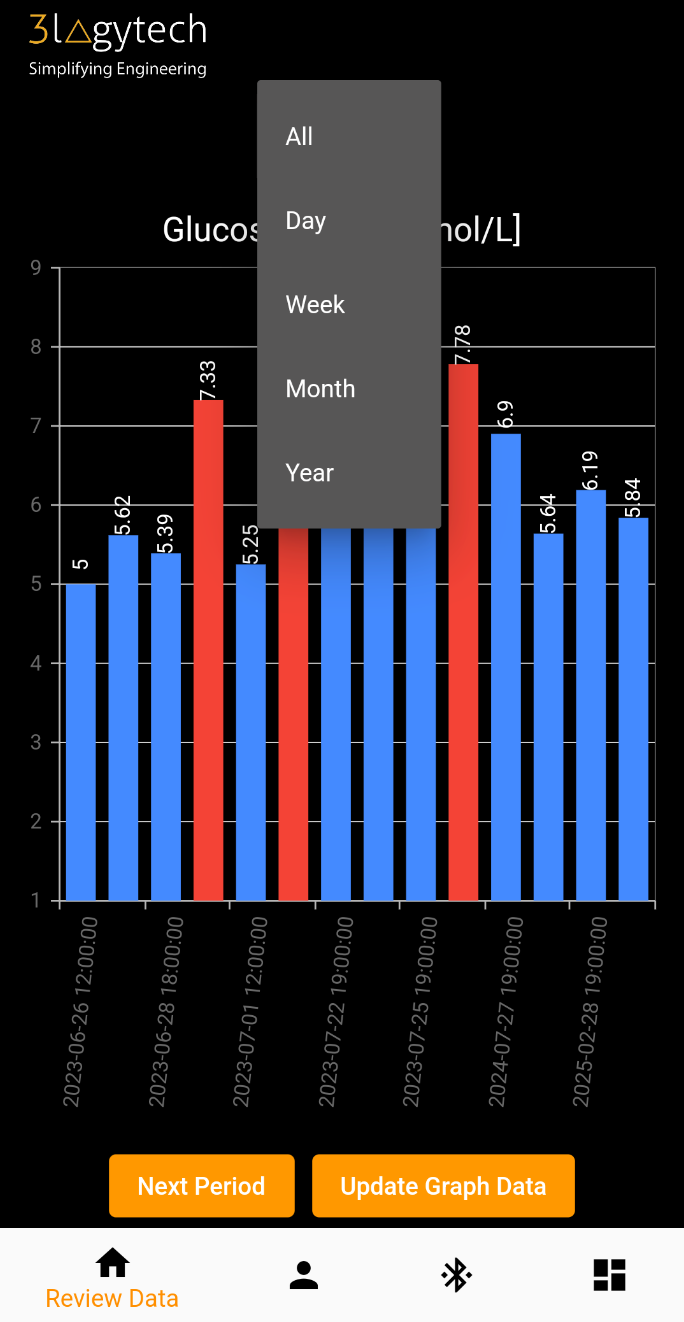
\includegraphics[scale=0.5]{graph_filter-options.png}
        \caption{Graph's filtering options}
        \label{fig:graph2}
    \end{subfigure}
\end{figure}
\begin{figure}[h]
\ContinuedFloat
    \begin{subfigure}{0.45\textwidth}
        \centering
        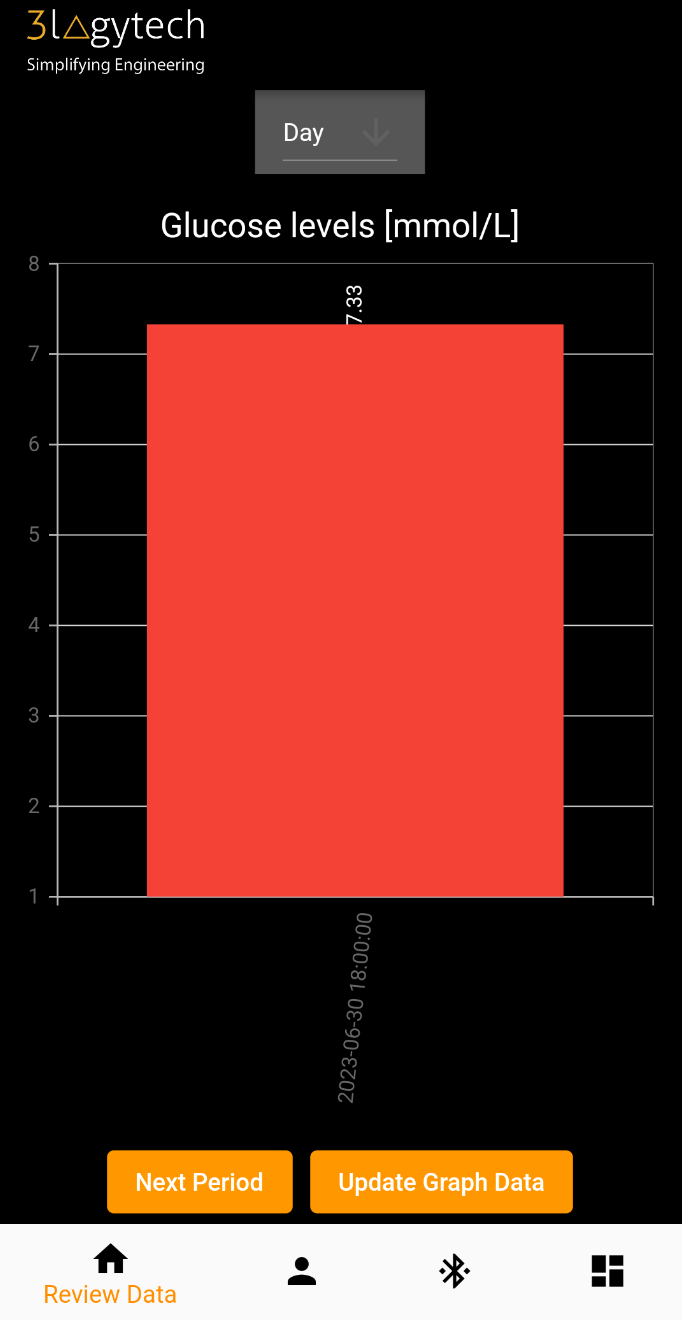
\includegraphics[scale=0.47]{graph_day.png}
        \caption{Data filtered by day}
        \label{fig:graph3}
    \end{subfigure}
    \begin{subfigure}{0.45\textwidth}
        \centering
        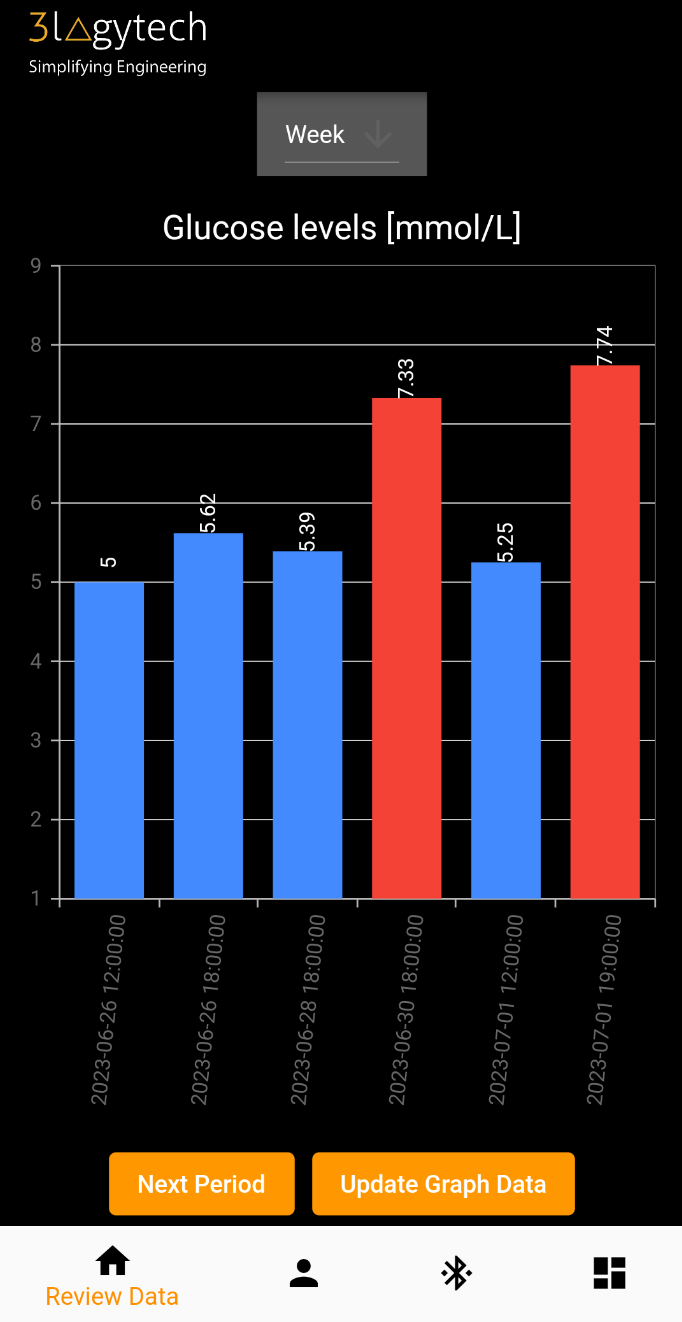
\includegraphics[scale=0.47]{graph_week.png}
        \caption{Data filtered by week}
        \label{fig:graph4}
    \end{subfigure}
\end{figure}
\begin{figure}[h]
\ContinuedFloat
    \begin{subfigure}{0.45\textwidth}
        \centering
        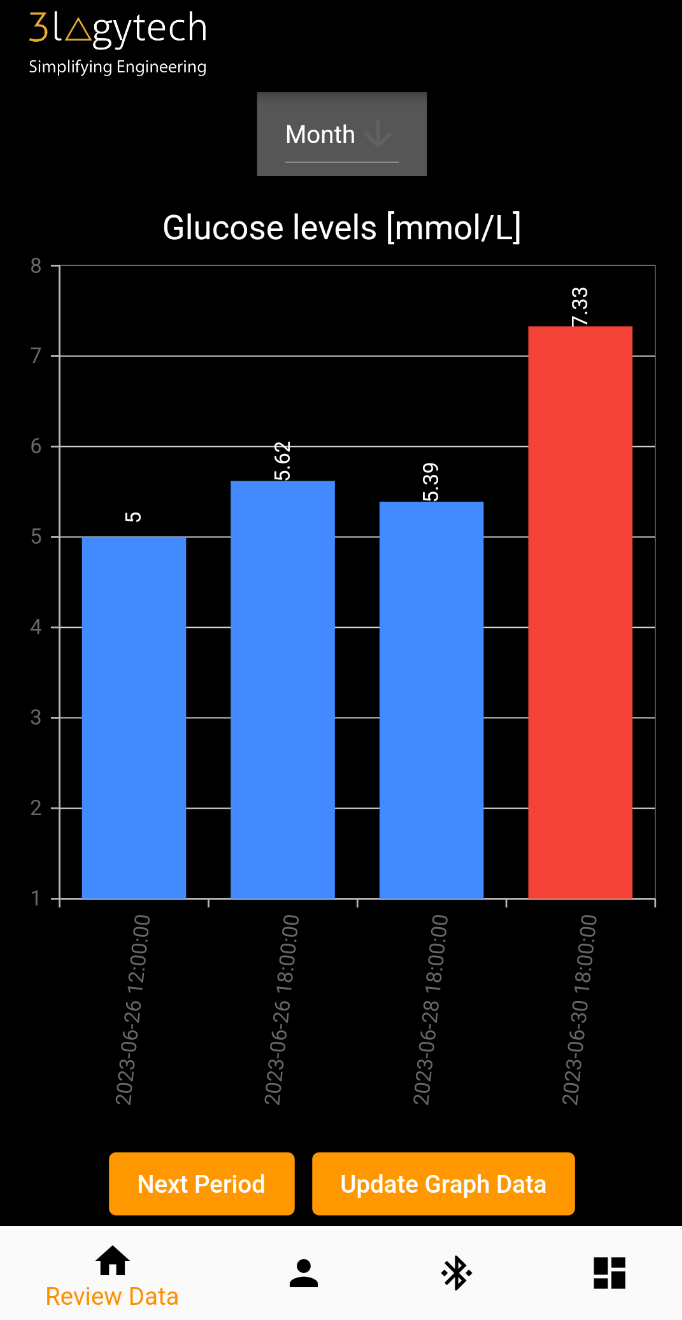
\includegraphics[scale=0.47]{graph_month.png}
        \caption{Data filtered by month}
        \label{fig:graph5}
    \end{subfigure}
    \begin{subfigure}{0.45\textwidth}
        \centering
        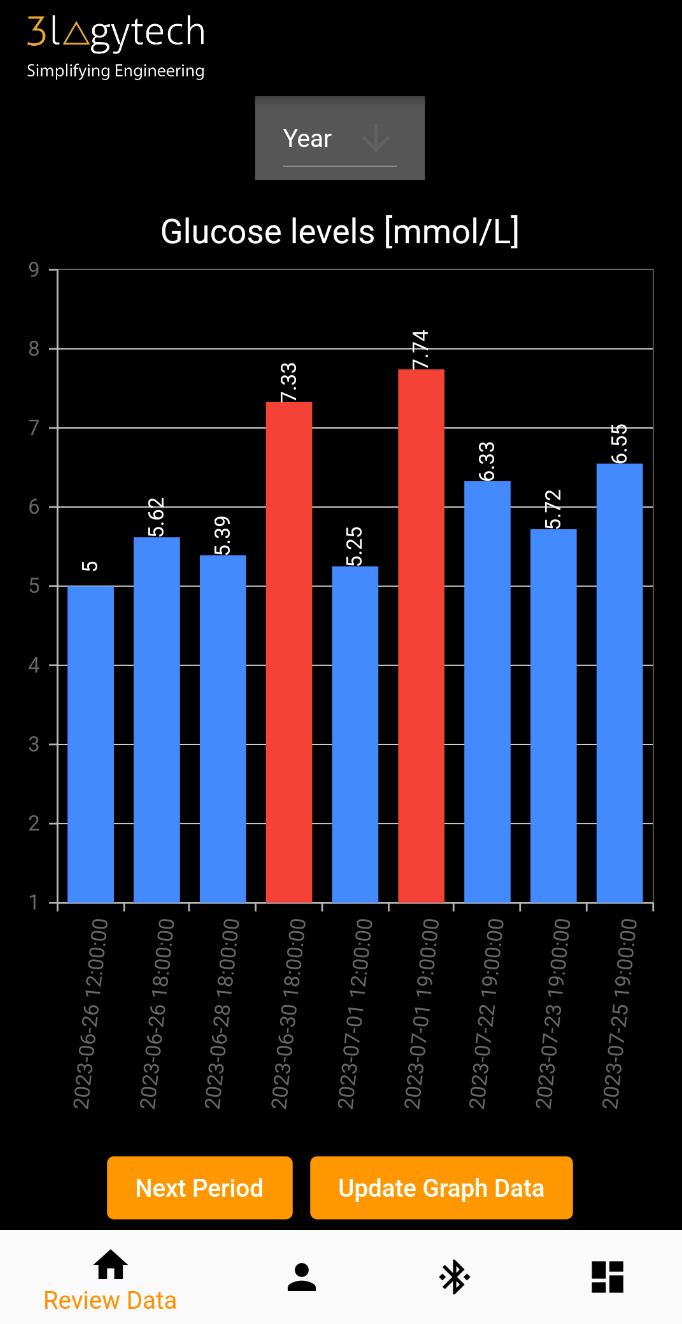
\includegraphics[scale=0.47]{graph_year.png}
        \caption{Data filtered by year}
        \label{fig:graph6}
    \end{subfigure}
\end{figure}

\clearpage
\section{Hardware Interfaces}
The app interacts with the following hardware components:
\begin{itemize}
    \item Glucometer device
    \begin{itemize}
        \item The app establishes connection with a compatible glucometer device via BLE.
        \item A compatible glucometer is one that contains "BGL" string in the name, eg. "BGL100", belonging to Trilogy Technologies.
        \item The app communicates with the glucometer to retrieve biodata.
    \end{itemize}
\end{itemize}

\section{Software Interfaces}
The app interacts with the following software components:
\begin{itemize}
    \item Operating system
    \begin{itemize}
        \item The app is designed to run on Android (version 8.0 or higher) and iOS (version 11.0 or higher).
    \end{itemize}
    \item Third-party libraries
    The app incorporates several third-party packages.
    \begin{itemize}
        \item app\_settings (version 4.2.0): Opens device settings page.
        \item csv (version 5.0.2): Enables reading and writing of CSV files for import and export functions.
        \item cupertino\_icons (version 1.0.5): Provides a collection of Cupertino-style icons for use in the app's user interface.
        \item device\_info\_plus (version 8.0.0): Retrieves device-specific information such as model, operating system and hardware details.
        \item excel (version 2.1.0): Enables reading and writing of Excel files for import and export functions.
        \item flutter\_background\_service (version 3.0.1): Allows the app to run in the background.
        \item flutter\_blue\_plus (version 1.4.0): Provides Bluetooth functionality and enables communication with Bluetooth devices.
        \item flutter\_email\_sender (version 5.2.0): Enables sending of emails from within the app using the device's local email application.
        \item flutter\_launcher\_icons (version 0.13.1): Simplifies the process of generating an app launcher icon for different platforms.
        \item flutter\_native\_splash (version 2.2.9): Simplifies the generation of native splash screens for the app on different platforms.
        \item fluttertoast (version 8.2.1): Displays toast messages on the screen after certain actions.
        \item intl (version 0.18.0): Offers internationalisation and localisation support for the app's user interface.
        \item path\_provider (version 2.0.15): Retrieves the file system paths for various platform-specific locations, enabling files to be retrieved and saved.
        \item permission\_handler (version 10.2.0): Handles runtime permissions, to provide users with the option to grant or deny specific permissions.
        \item shared\_preferences (version 2.1.1): Stores and retrieves the app preferences and settings in a persistent manner.
        \item sqflite (version 2.2.8+4): Provides SQLite database support for the app, for storing of data locally.
        \item syncfusion\_flutter\_charts (version 21.2.4): Enables visualisation of blood glucose trends and generate informative graphs.
    \end{itemize}
\end{itemize}

\chapter{System Features}

\section{Personal Information page}
\begin{itemize}
    \item App must be able to accept user input.
    \item App must be able to store user data.
    \item App must allow users to change language.
\end{itemize}
\section{Find Devices page}
\begin{itemize}
    \item App must be able to scan and detect compatible glucometer devices via BLE.
    \item App must give the user an option to start and stop scanning for devices.
    \item App must be able to display the data retrieved from the glucometer device.
    \item App must give the user an option to view the data in a more visually appealing dashboard.
\end{itemize}
\section{Dashboard page}
\begin{itemize}
    \item The dashboard must be visually appealing.
    \item The dashboard must have big fonts for easy viewing.
    \item The dashboard must be display data labelled with the appropriate units of measurement.
\end{itemize}
\section{Graph page}
The graph used in the app is a bar graph.
\begin{itemize}
    \item The graph page must provide a graph for the user to view their glucose level trends.
    \item The graph must only be displayed if the database is nonempty.
    \item The graph should provide a function for the user to view their data at specific time periods eg. day, week, month, year, all.
    \item The bars in the graph should be a different colour (red) to highlight to the user that the glucose level is above the threshold.
\end{itemize}

\chapter{Other Nonfunctional Requirements}
\section{Performance Requirements}
\begin{itemize}
    \item The app must not crash when the user opens it.
    \item The app must be able to display each page within 3 seconds of the user opening it.
\end{itemize}
\section{Usability Requirements}
\begin{itemize}
    \item The app design must be intuitive for ease of navigation.
    \item All features of the app must be clearly displayed.
    \item The app must offer insightful information to the user about their health or glucose level management.
    \item The app must provide necessary feedback to the user if there are invalid inputs.
    \item The app must display appropriate error messages when certain processes fail or when vital system permissions are not enabled.
    \item The app must support English languauge.
\end{itemize}
\section{Reliability Requirements}
\begin{itemize}
    \item The app must not break due to any invalid input.
    \item The app must have all features available at all times, provided the user's device is at 100\% functionality.
\end{itemize}
\section{Security Requirements}
\begin{itemize}
    \item User data should not be disclosed without their consent.
    \item User data must not be seen or accessible by other users, except the user's own certified medical professional(s).
    \item All data must be deleted when the user chooses to delete it.
\end{itemize}
\section{Maintainability Requirements}
\begin{itemize}
    \item Maintenance shall be conducted regularly to ensure the app and its' dependencies are up to date.
    \item Security or software updates shall be rolled out periodically and when necessary.
\end{itemize}
\section{Software Quality Attributes}
The app adheres to good software engineering design principles of
\begin{itemize}
    \item Good design
    \begin{itemize}
        \item Reusability of features
        \begin{itemize}
            \item Methods for user account creation and storing of user data in a database can be reused for another project.
        \end{itemize}
    \end{itemize}
    \begin{itemize}
        \item Testability of features
        \begin{itemize}
            \item Each feature can be tested independently.
        \end{itemize}
    \end{itemize}
    \begin{itemize}
        \item Maintainability of features
        \begin{itemize}
            \item Ensured readability of code.
            \item Included comments to help anyone else reading the source code understand what the function does.
        \end{itemize}
    \end{itemize}
    \begin{itemize}
        \item Extensibility of features
        \begin{itemize}
            \item The flexible architecture allows new modules or components to be added without affecting the existing system.
        \end{itemize}
    \end{itemize}
    \item Design Patterns
    \begin{itemize}
        \item Single responsibility principle
        \begin{itemize}
            \item Our application is broken down into smaller, individual functions, each with a single responsibility.
            \item Improves reusability as each function can be reused in other modules.
            \item Improves maintainability as each function is less likely to affect other functions.
        \end{itemize}
    \end{itemize}
    \item Design Principles
    \begin{itemize}
        \item High cohesion
        \begin{itemize}
            \item The modules in the system have a single, well-defined responsibility.
        \end{itemize}
        \item Low coupling
        \begin{itemize}
            \item Changes in one module will not affect other functions.
            \item Modules do not have overlapping responsibilities and does not affect each other at all.
        \end{itemize}
        \item Open-Closed
        \begin{itemize}
            \item Extension of current functions is possible.
        \end{itemize}
        \item Separation of concerns
        \begin{itemize}
            \item The code is more readable since all the components do not have overlapping functionalities.
        \end{itemize}
    \end{itemize}
\end{itemize}


\chapter{Appendix A: Installation}
\section{Setup}
To run this app on your local machine, follow these steps:
\begin{enumerate}
    \item Ensure you have Flutter installed on your system. If not, you can install it from
    the official Flutter website: \url{https://flutter.dev/docs/get-started/install}.
    
    \item To build: You'll need \href{https://developer.android.com/studio/}{Android Studio},
    \href{https://developer.apple.com/xcode/}{Xcode}, \href{https://docs.expo.io/workflow/ios-simulator/}{iOS Simulator}, and \href{https://cocoapods.org/}{Cocoapods}. You will need to sign in to your Apple Developer account to run the app on your device.
\end{enumerate}

    From your command line:
    \begin{verbatim}
        # Go into the folder
        $ cd max_heart_reader
        
        # Install dependencies
        $ flutter clean
        $ flutter pub get
        
        # Run the app
        $ flutter run
    \end{verbatim}

    \begin{quote}
        \textbf{Note:} If you're testing on iOS, \href{https://docs.flutter.dev/testing/build-modes}{see this guide}. The default mode is \texttt{--debug} where the app cannot run in standalone mode.
    \end{quote}
    
    \subsection*{Build for iOS: Create Podfile}
    
    To begin, create a \texttt{Podfile} in the root directory of your iOS project. The \texttt{Podfile} specifies the dependencies for your project. Open the terminal and navigate to your project's root directory:
    
    
To begin, create a `Podfile` in the root directory of your iOS project. The `Podfile` specifies the dependencies for your project.
Open the terminal and navigate to your project's root directory:
    \begin{verbatim}
        cd /path/to/YourProjectIOSFolder

        # If Podfile does not exist
        touch Podfile

        pod install

        # Open .xcworkspace
        open Runner.xcworkspace
        
        # Click on the play button in Xcode to build and run the app.
    \end{verbatim}
\section{Internationlization}
The app containing the code for the different languages is located in the \textit{lib/l10n} folder. \textit{l10n} is the naming convention for localization. The number 10 is the number of letters
between the \textit{l} and \textit{n} in the word localization.
\newline
\newline
To add or edit more languages for the app, follow these \href{https://docs.flutter.dev/accessibility-and-localization/internationalization}{steps} as taken from the official Flutter documentation.
\newline
The steps listed more than suffice for the purposes of this app.
The l10n.yaml file is already created, which tells the compiler where to find the \textit{.arb} files and will auto generate the required \textit{.dart} files.
\newline
\newline
To generate new \textit{app_localizations_\{YourLocaleHere\}.dart} files, run in command line:
\begin{verbatim}
    flutter gen-l10n
\end{verbatim}


\chapter{Appendix B: Troubleshooting}
This page lists the common problems encountered during the development of the app and how they can be resolved. Do note that this list is not exhaustive and there may be other solutions to the problems.
\begin{itemize}
    \item Change the name of the app:
    \url{https://stackoverflow.com/questions/49353199/how-can-i-change-the-app-display-name-build-with-flutter}
    
    \item Change the icon of the app:
    \url{https://pub.dev/packages/flutter_launcher_icons}
    
    \item Change applicationId and bundle identifier to prevent overwrite:
    \url{https://stackoverflow.com/questions/58229150/how-to-run-a-copy-of-flutter-project-without-overwriting-the-existing-app}
    
    \item Run background service to keep uploading data when app is turned off:
    \url{https://pub.dev/packages/flutter_background_service}
    
    \item Splash screen:
    \url{https://pub.dev/packages/flutter_native_splash/example}
    \url{https://www.youtube.com/watch?v=dB0dOnc2k10&ab_channel=JohannesMilke}
    
    \item Loading screen:
    \url{https://codewithflutter.com/create-splash-screen-in-flutter-app/}
    
    \item Enable and Check Location Permissions:
    \url{https://pub.dev/packages/permission_handler}
    
    \item To compile on iOS:
    \begin{itemize}
        \item nil:NilClass for Flutter App / CocoaPod Error:
        \url{https://stackoverflow.com/questions/67443265/error-regarding-undefined-method-map-for-nilnilclass-for-flutter-app-cocoap}
        \item Make sure to click "Trust" on iPhone when connecting iPhone to PC
        \item bundle ID error:
        \url{https://stackoverflow.com/questions/51098042/how-to-get-bundle-id-in-flutter}
        \item "Untrusted Developer" after XCode build is done:
        \url{https://developer.apple.com/forums/thread/660288}
        General -> VPN \& Device Management -> Developer App -> Verify
        \item Make sure that the sign in is successful in XCode:
        \url{https://docs.flutter.dev/deployment/ios}
        Go to XCode -> Runner -> Signing \& Capabilities -> Team -> Select apple developer account
        \item Dart SDK is not configured:
        \url{https://stackoverflow.com/questions/48650831/dart-sdk-is-not-configured}
        Click on settings gear (IDE and Project Settings) -> Preferences -> Language \& Framework -> Flutter -> choose flutter SDK
        \item (when compiling Android app on Macbook): Execution failed for task ':app-compileFlutterBuildDebug':
        \url{https://stackoverflow.com/questions/61930007/how-to-solve-execution-failed-for-task-appcompileflutterbuilddebug}
    \end{itemize}
\end{itemize}

\end{document}